% !TEX root = replicas_draft.tex


\section{Single interval at zero temperature}
\la{sec:OneZero}

There is a very simple version of the information paradox at zero temperature \cite{Almheiri:2019yqk}. Consider the region $R$ in fig.~\ref{fig:zerotemp-lorentzian}. Ignoring gravity, the von Neumann entropy of the quantum fields on this region is infrared divergent. This is the Hawking-like calculation of the entropy using quantum field theory on a fixed background.

The state of the quantum fields on a full Cauchy slice is pure. However, the AdS$_2$ region is supposed to be a quantum system with $e^{S_0}$ states. This is a contradiction, because it is impossible for the finite states in the AdS$_2$ region to purify the IR-divergent entropy of region $R$. The UV divergence is not relevant to this issue because it is purified by CFT modes very close to the endpoint.

This is resolved by including an island, as in fig.~\ref{fig:zerotemp-lorentzian} \cite{Almheiri:2019yqk}. We will describe briefly how this is reproduced from a replica wormhole. This doesn't require any new calculations because we can take the limit $\beta \to \infty$ in the finite temperature result.  The pictures, however, are slightly different, because the replica geometries degenerate in this limit and the topology changes.

\begin{figure}
\begin{center}
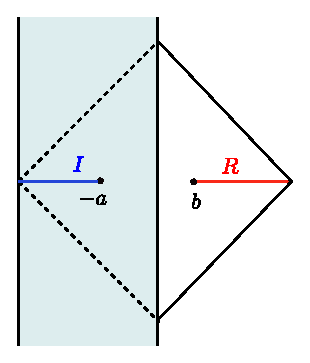
\includegraphics[scale=1.0]{figures/zerotemp-lorentzian.pdf}
\end{center}
\caption{\small An information puzzle at zero temperature, with AdS$_2$ on the left and flat space on the right. The naive calculation of matter entropy in region $R$ is infrared-divergent, but this cannot be purified by quantum gravity in AdS$_2$. This is resolved by including the island, $I$.}\label{fig:zerotemp-lorentzian}
\end{figure}

\subsection{Quantum extremal surface}
The metric and dilaton for the zero-temperature solution are 
\be
ds^2_{in} = \frac{4 dy d\by }{(y + \by)^2} \ , \qquad \qquad \phi =- \frac{2\phi_r}{y + \by} \ , ~~~~~~~~y = \sigma + i \tau 
\ee
with $\sigma<0$. As before we glue it to flat space $dy d\bar y $ at $\sigma =0$. The region $R$ and the island $I$ are the intervals
\be
I: \quad y \in (-\infty, -a] , \qquad
R: \quad y \in [b,\infty)
\ee
at $t=0$. 
The generalized entropy, including the island, is
\be
S_{\rm gen}(I \cup R) = \frac{\phi_r}{a} + \frac{c}{6}\log \frac{(a+b)^2}{a} \ .
\ee
Setting $\p_a S_{\rm gen} = 0$ gives the position of the QES,
\be\label{zerotempQES}
a = \frac{1}{2}(k + b + \sqrt{b^2 + 6bk + k^2})  \ , \quad k \equiv \frac{6\phi_r}{c} \ .
\ee

\subsection{Replica wormholes at zero temperature}
The replica partition function $\Tr (\rho_A)^n$ is given by the path integral in fig.~\ref{fig:zerotemp-euclidean}. The boundary condition for the gravity region is $n$ copies of the real line. The Hawking saddle fills in the gravity region with $n$ independent copies of $\mathbb{H}_2$. The replica wormhole, shown in the figure, fills in the gravity region with a single copy of $\mathbb{H}_2$. To see all $n$ sheets of the gravity region, we go to the uniformizing coordinate
\be
\widetilde{w} = \left(\frac{a+y}{a-y } \right)^{1/n} \ .
\ee
This maps the full gravity region to a single hyperbolic disk, $|\widetilde{w}| < 1$. This disk is a wormhole connecting $n$ copies of flat space. The $n^{th}$ copy is glued to the segment with arg $\widetilde w \in [-\frac{\pi}{n}, \frac{\pi}{n}]$.

\begin{figure}
\begin{center}
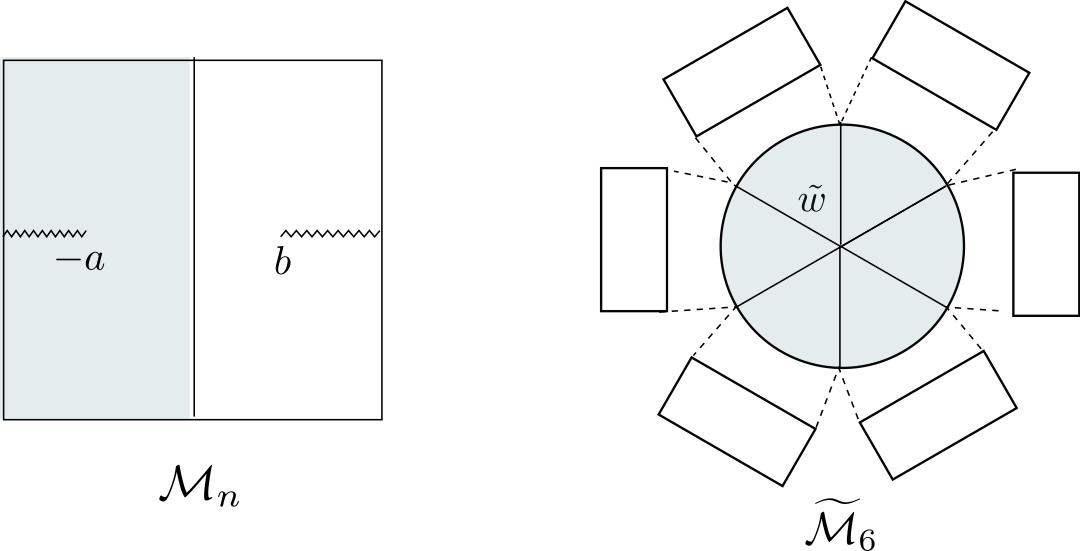
\includegraphics[scale=0.5]{figures/zerotemp-euclidean.png}
\end{center}
\caption{\small Replica wormhole at zero temperature. On the right, the disk is glued to $n$ copies of the half-plane, as indicated by the dashed lines. } \label{fig:zerotemp-euclidean}
\end{figure}

The equation of motion, and the answer for the position of the QES, is found by taking $\beta \to \infty$ in the results of section \ref{sec:SingleInterval}. This of course agrees with \eqref{zerotempQES}. (It is also possible to solve this problem directly at zero temperature, but we found it easier to treat the welding problem at finite temperature where the gluing is compact. In the end, the welding effects drop out in the determination of the position of the QES, as we saw below \eqref{hilbertp}.)







